\section{Техническое задание}
\subsection{Основание для разработки}

Основанием для разработки информационно-вычислительной системы является задание на выпускную квалификационную работу по программе бакалавра «Программное обеспечение для управления работой центра здорового питания» согласно приказу №5197-с от 13.11.2023. «Об утверждении тем выпускных квалификационных работ и руководителей выпускных квалификационных работ».

Необходимо спроектировать и разработать сайт, который должен способствовать упрощению работы для врачей-диетологов в центре здорового питания.

Интернет-сайт представляет собой набор взаимосвязанных электронных страниц, которые сгруппированы по разделам, содержащие текстовую, графическую. Сайт располагается в Интернете по определенному адресу – доменному имени сайта в виде www.имя\_сайта.ru. Каждая страница web-сайта – это текстовый документ, написанный на языке программирования (HTML, CSS, JavaScript и т.д.).

\subsection{Цель и назначение разработки}

Программный продукт предназначен для компаний связанных со здоровым питанием, чтобы упростить рабочий процесс.Данный программный продукт предназначен для использования в различного рода коммерческих и бюджетных организациях.

Задачами данной разработки являются:
\begin{itemize}
\item создание разделов сайта;
\item реализация формы для входа;
\item реализация формы для регистрации пациента;
\item реализация формы карты пациента;
\item реализация формы для назначения диеты;
\item реализация калькулятора подсчета КБЖУ;
\item создание удобного поиска по сайту.
\end{itemize}

\subsection{Требования пользователя к интерфейсу web-сайта}

Сайт должен включать в себя:
\begin{itemize}
    \item авторизацию;
    \item навигацию по разделам;
    \item регистрация пациента;
    \item просмотр списка пациентов;
    \item просмотр карты пациента;
    \item просмотр списка продуктов с пищевой ценностью;
    \item просмотр списка болезней желудочно-кишечного тракта.
\end{itemize}

Для взаимодействия с системой должен быть разработан интерфейс по макетам представленных на рисунках.

Макет страницы "Авторизация" представлен на рисунке ~\ref{fig:image}.
\begin{figure}[th]
	\centering
	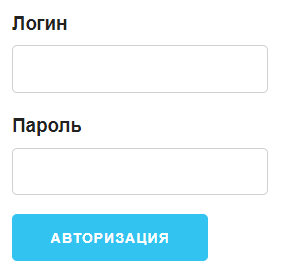
\includegraphics[width=1\linewidth]{images/Авторизация}
	\caption{Макет страницы "Авторизация"}
	\label{fig:image}
\end{figure}

Макет страницы навигационной панели представлена на рисунке ~\ref{fig:imagen}.
\begin{figure}[H]
	\centering
	
\includegraphics[width=1\linewidth]{images/Нав.панель}
	\caption{Навигационная панель}
	\label{fig:imagen}
\end{figure}

Макет страницы регистрация пациента представлена на рисунке ~\ref{fig:imagep}.
\begin{figure}[H]
	\centering
	\includegraphics[width=1\linewidth]{"images/Регистрация пациента"}
	\caption{Регистрация пациента}
	\label{fig:imagep}
\end{figure}

Макет страницы список пациентов представлена на рисунке ~\ref{fig:images}.
\begin{figure}[H]
	\centering
	\includegraphics[width=1\linewidth]{"images/Список пациентов"}
	\caption{Список пациентов}
	\label{fig:images}
\end{figure}

Макет страницы информация о пациенте представлена на рисунке ~\ref{fig:imagein}.
\begin{figure}[H]
	\centering
	\includegraphics[width=1\linewidth]{"images/Инфа о пациенте"}
	\caption{Список пациентов}
	\label{fig:imagein}
\end{figure}

Макет страницы списка продуктов представлена на рисунке ~\ref{fig:imagepr}.
\begin{figure}[H]
	\centering
	\includegraphics[width=1\linewidth]{"images/Список продуктов"}
	\caption{Список продуктов}
	\label{fig:imagepr}
\end{figure}

Макет страницы списка болезней представлена на рисунке ~\ref{fig:imagebl}.
\begin{figure}[H]
	\centering
	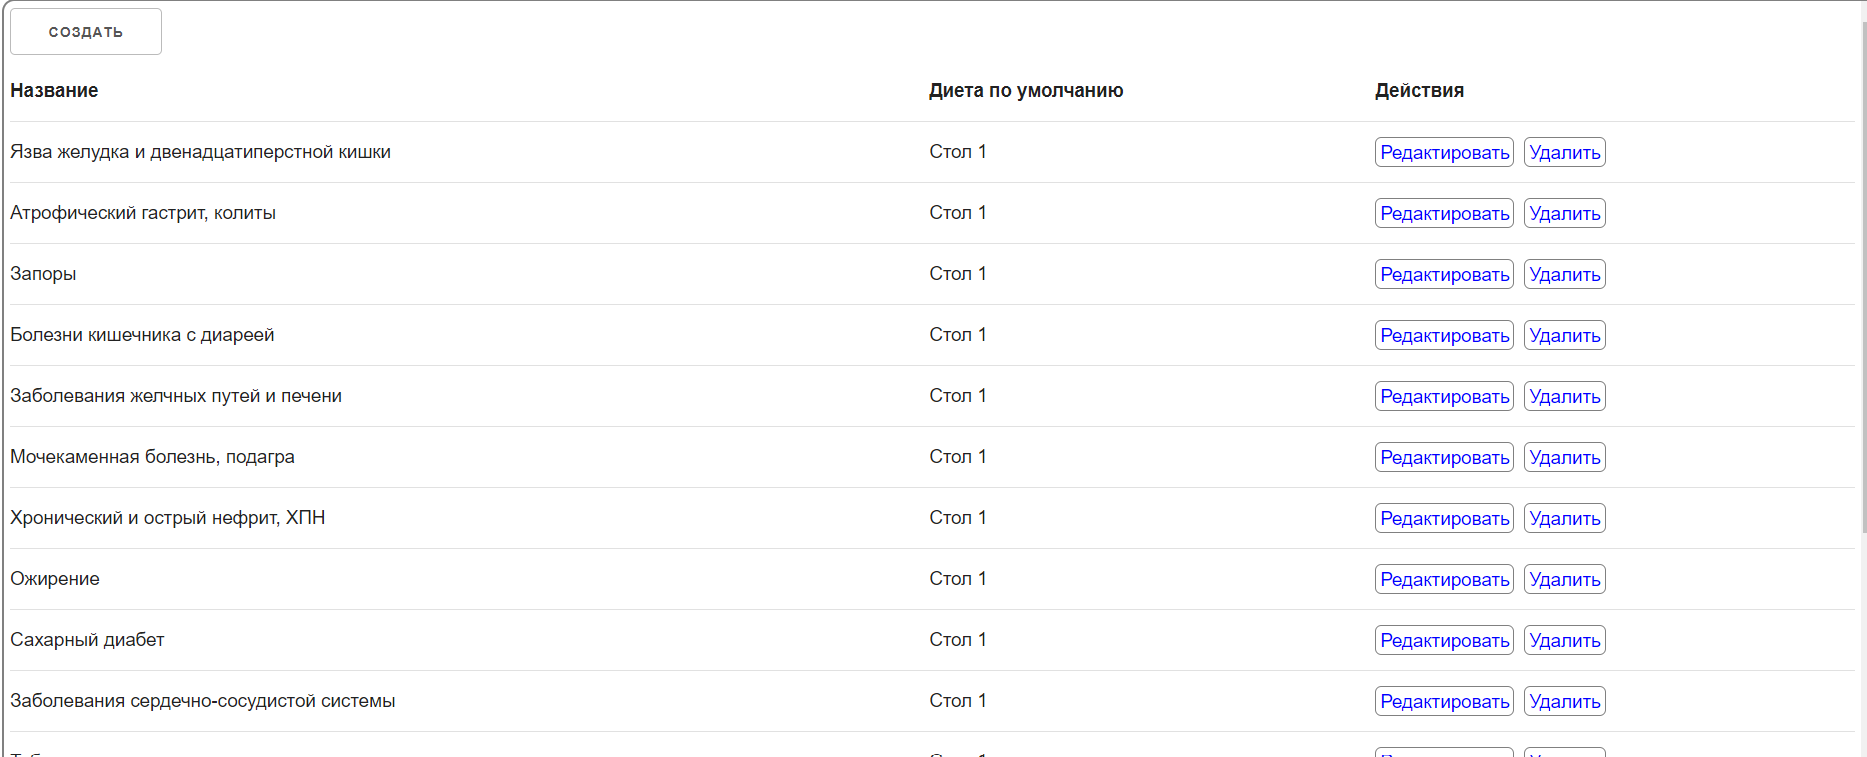
\includegraphics[width=1\linewidth]{images/Болезни}
	\caption{Список болезней}
	\label{fig:imagebl}
\end{figure}

%\vspace{-\figureaboveskip} % двойной отступ не нужен (можно использовать, если раздел заканчивается картинкой)

\subsection{Функциональные требования к программной системе}

Разрабатываемая система должна иметь несколько ролей
пользователей:

\begin{itemize}
	\item администратор;
	\item врач.
\end{itemize}

Для администратора должны быть предусмотрены следующие функции в разрабатываемой системе: 

\begin{itemize}
	\item авторизация;
	\item просмотр списка врачей;
	\item создание пользователя;
	\item редактирование пользователя;
	\item удаление пользователя;
	\item просмотр списка продуктов;
	\item добавление продукта;
	\item редактирование продукта;
	\item удаление продукта;
	\item просмотр списка болезней;
	\item добавление болезни;
	\item редактирование болезни;
	\item удаление болезни;
	\item просмотр списка пациентов;
	\item просмотр списка диет;
	\item добавление диеты;
	\item редактирование диеты;
	\item удаление диеты;
	\item Выход из системы.
\end{itemize}

Для врача должны быть предусмотрены следующие функции в разрабатываемой системе:

\begin{itemize}
	\item авторизация;
	\item просмотр списка продуктов;
	\item добавление продукта;
	\item редактирование продукта;
	\item удаление продукта;
	\item просмотр списка болезней;
	\item добавление болезни;
	\item редактирование болезни;
	\item удаление болезни;
	\item просмотр списка пациентов;
	\item регистрация пациента;
	\item редактирование информации о пациенте;
	\item назначение диеты пациенту;
	\item добавление болезни пациенту;
	\item удаление пациента;
	\item просмотр списка диет;
	\item добавление диеты;
	\item редактирование диеты;
	\item удаление диеты;
	\item Выход из системы.
	\end{itemize}
	
Требования к входным и выходным данным для описанных функций разрабатываемой информационно-вычислительной системы:

Данные функции "Авторизация"

Входными данными для данной функции является логин и пароль существующего аккаунта.

Выходными данными для данной функции является токен верификации запросов.

Данные функции "Выход"

Входными данными для данной функции является токен верификации.

Выходными данными для данной функции является ответ системы об успешном выходе из аккаунта.

Данные функции "Просмотр списка продуктов"

Входными данными для данной функции является токен авторизации.

Выходными данными для данной функции является список продуктов.

Данные функции "Добавление продукта"

Входными данными для данной функции является наименование продукта и КБЖУ.

Выходными данными для данной функции является является обновленное содержимое списка.

Данные функции "Редактирование продукта"

Входными данными для данной функции является id, название, КБЖУ.

Выходными данными для данной функции является содержимое обновленного списка.

Данные функции "Удаление продукта"

Входными данными для данной функции является текущая директория и наименование удаляемого продукта.

Выходными данными для данной функции является обновленное содержимое данной директории.

Данные функции "Просмотр списка болезней"

Входными данными для данной функции является токен авторизации.

Выходными данными для данной функции является список болезней.

Данные функции "Добавление болезни"

Входными данными для данной функции является наименование болезни, назначаемая диета.

Выходными данными для данной функции является обновленный список болезней.

Данные функции "Редактирование болезни"

Входными данными для данной функции является id, название, назначенную диету.

Выходными данными для данной функции является обновленный список болезней.

Данные функции "Удаление болезни"

Входными данными для данной функции является id, наименование удаляемой болезни.

Выходными данными для данной функции является обновленный список болезней.

Данные функции "Просмотр список пациентов"

Входными данными для данной функции является токен авторизации.

Выходными данными для данной функции является список пациентов.

Данные функции "Регистрация пациента"

Входными данными для данной функции является id, ФИО, возраст, пол, вес, активность, цель.

Выходными данными для данной функции является обновленный список пациентов.

Данные функции "Редактирование информации о пациенте"

Входными данными для данной функции является id, ФИО, возраст, пол, вес, активность, цель.

Выходными данными для данной функции является обновленный список пациентов.

Данные функции "Назначение диеты пациенту"

Входными данными для данной функции является DietID, название диеты, список продуктов.

Выходными данными для данной функции является обновленный список диет.

Данные функции "Добавление болезни пациенту"

Входными данными для данной функции является DiseaseID, название болезни.

Выходными данными для данной функции является обновленный список болезни.

Данные функции "Удаление пациента"

Входными данными для данной функции является id, фио, возраст, пол, вес, активность, цель.

Выходными данными для данной функции является обновленный список пациентов.

Данные функции "Просмотр списка диет"

Входными данными для данной функции является токен авторизации.

Выходными данными для данной функции является список диет.

Данные функции "Добавление диеты"

Входными данными для данной функции является id, наименование, продукты, болезни.

Выходными данными для данной функции является обновленный список диет.

Данные функции "Редактирование диеты"

Входными данными для данной функции является id, наименование, продукты, болезни.

Выходными данными для данной функции является обновленный список диет.

Данные функции "Удаление диеты"

Входными данными для данной функции является id, наименование, продукты, болезни.

Выходными данными для данной функции является обновленный список диет.


\subsection{Нефункциональные требования к программной системе}

Требования к аппаратной совместимости: 

\begin{itemize}
	\item оперативная память: 2 ГБ;
	\item минимальное количество места на жестком диск: 5 ГБ;
	\item частота процессора 2 Ггц, число ядер 4.
\end{itemize}

Требования к программной совместимости:

\begin{itemize}
	\item операционная система Linux с версией ядра не ниже 4, либо Windows 10 с версией не ниже 2004;
\end{itemize}

Требования к производительности. Отклик программной системы на действия должен быть немедленным и не превышать 100 миллисекунд. Обработка всех документов происходит в порядке очереди, в то же время запросов пользователей обрабатываются в асинхронном режиме для максимальной отзывчивости системы.

\subsection{Требования к оформлению документации}

Оформление документации должно осуществляться в соответствии с ГОСТами единой системы программной документации, единой системы конструкторской документации.